\documentclass{report}
\usepackage{fancyhdr} % Required for custom headers
\usepackage{lastpage} % Required to determine the last page for the footer
\usepackage{extramarks} % Required for headers and footers
\usepackage{graphicx} % Required to insert images
%\usepackage{lipsum} % Used for inserting dummy 'Lorem ipsum' text into the template
\usepackage{amsmath}
\usepackage{graphicx} 
\usepackage{float}
%\usepackage{amsfont}
%\usepackage{amssymb}

\usepackage{multicol}
% Margins
\topmargin=-0.5in
\evensidemargin=0in
\oddsidemargin=-0.5in
\textwidth=7.5in
\textheight=9.0in
\headsep=0.25in 


\pagestyle{fancy}

%\rhead{\textbf{Marshall's Recipes}} % Top right header
%\lhead{\textbf{Curry Stir Fry}}
%\chead{ }
%\title{Curry Stir Fry}

\begin{document}
%\vspace{8mm}
%\textbf{PRELIMINARIES:}


\bigskip

\bigskip

\begin{multicols}{2}
\textbf{Ingredients}
\begin{itemize}
\item 2 quarts water
\item 8-10 lipton tea bags (regular black tea
\item 2 sticks of Cinnamon
\item 2 piece of star anise
\item 10 cardamon pods (split open)
\item $\frac{1}{4}$ tsp. ground nutmeg
\item 5-6 whole cloves
\item 2-3 whole allspice 
\item 1 can of evaporated milk\newline (480 kCal / 24 gP / 24 gF / 36 gC)
\item 3 bay leaves
\item 2 tbsp. balsamic vinegar
\item salt to taste
\item pepper to taste
\item 4 sprigs fresh thyme if available, otherwise dried thyme to taste
\item parmesan cheese to sprinkle on top 


\end{itemize}


\columnbreak
\textbf{Procedure:}
\medskip


\begin{enumerate}
\item \textbf{Note:} This recipe is portioned for approximately 6 mugs. 
\item Place spices in water and bring to boil. Simmer for 20-25 minutes. 

\item Add teabags and steep for 5-10 min.

\item Remove tea bags and squeeze with tongs to drain. 

\item Add evaporated milk and bring “almost” back to boil.

\item Turn off heat or reduce to very low, add sugar to taste.  



\begin{table}[H]
  \begin{center}
    \caption{Macro totals}
    \label{tab:table1}
    \begin{tabular}{c|c|c|c} % <-- Alignments: 1st column left, 2nd middle and 3rd right, with vertical lines in between
      \textbf{Calories} & \textbf{Protein} & \textbf{Fat} & \textbf{Carbs}\\
      \hline
      1814 kCal & 78 g & 63 g & 206 g\\
    \end{tabular}
  \end{center}
\end{table}
 
\end{enumerate}
\end{multicols}




%\begin{center}
%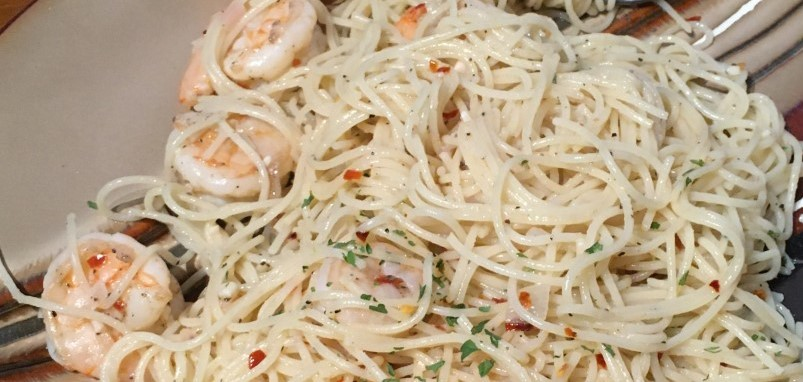
\includegraphics[scale=0.65]{Pasta/Shrimp Scampi/Shrimp Scampi.jpg}
%\end{center}


\end{document}